\newpage
\section{Installing the FTP Server Service and Wireshark}

\subsection{Activity}

\noindent {\bf{Bước 1:}} Khởi động Windows Server.

\noindent {\bf{Bước 2:}} Ở Server Manager, chọn \textbf{Manage} > \textbf{Add Roles and Features}. Khi gặp \textbf{Server Roles}, chọn \textbf{Web Server (IIS)}. Sau đó \textbf{Add Features}.

\begin{figure}[!htb]
    \centering
    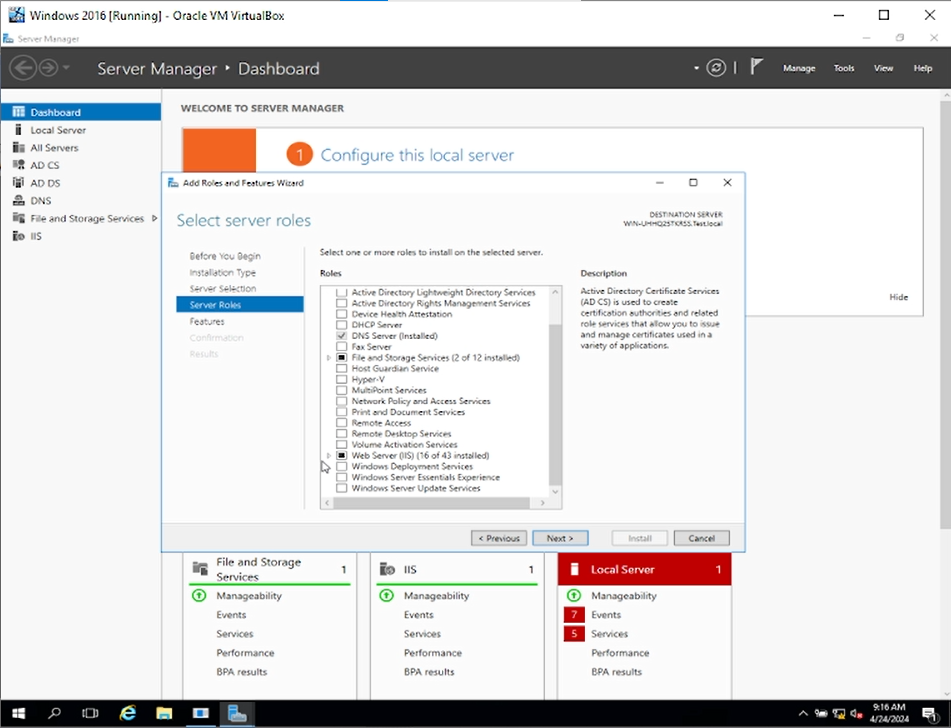
\includegraphics[width=0.7\linewidth]{figure//chapter9//lab9_2/setup_web_server.png}
    \caption{Chọn Web Server (IIS)}
    \label{fig:enter-label}
\end{figure}

\noindent {\bf{Bước 3:}} Tiếp tục tới \textbf{Role Services}, chọn \textbf{FTP Service}. Chọn \textbf{Install}.

\begin{figure}[!htb]
    \centering
    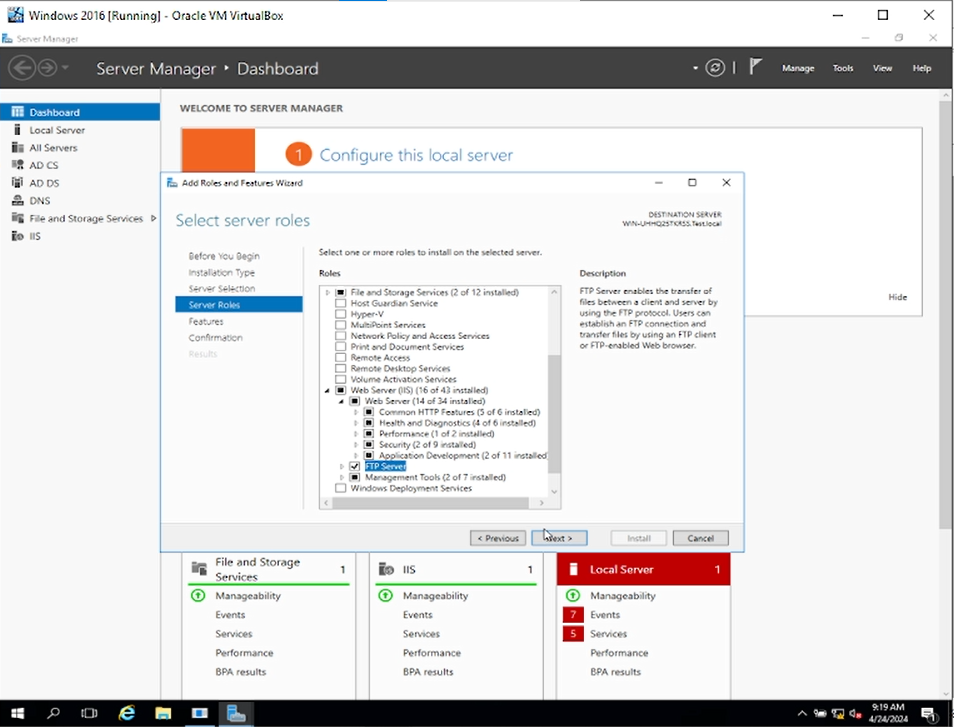
\includegraphics[width=0.7\linewidth]{figure//chapter9//lab9_2/ftp_server.png}
    \caption{Chọn FTP Server}
    \label{fig:enter-label}
\end{figure}

\noindent {\bf{Bước 4:}} Vào Internet Information Services (IIS) Manager. 

\begin{figure}[!htb]
    \centering
    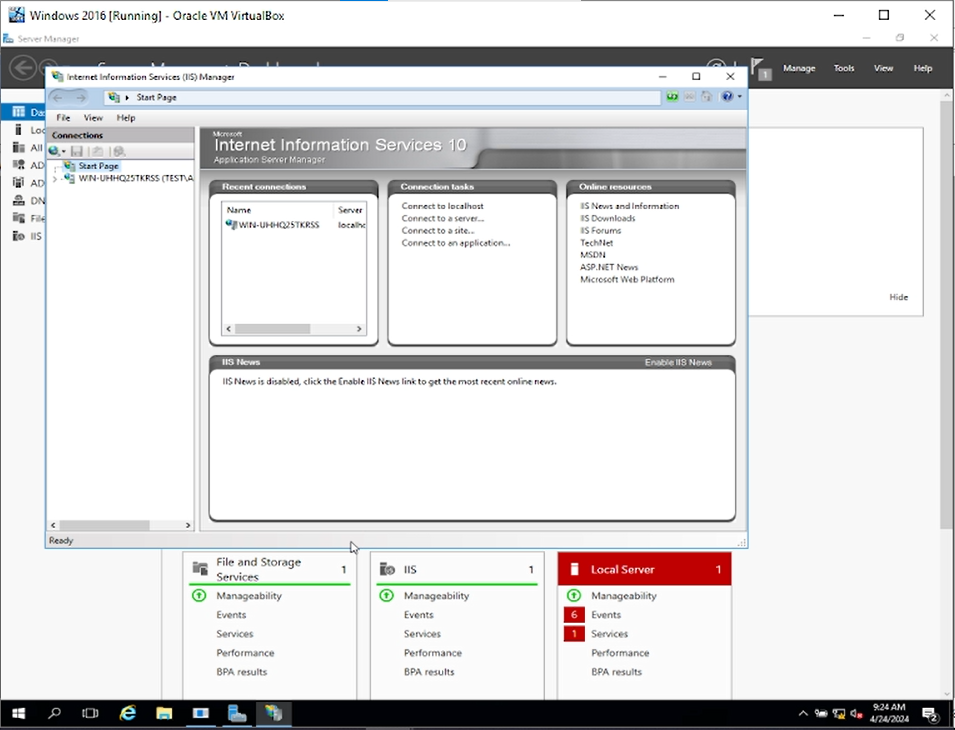
\includegraphics[width=0.8\linewidth]{figure//chapter9//lab9_2/iis.png}
    \caption{IIS Manager}
    \label{fig:enter-label}
\end{figure}

\noindent {\bf{Bước 5:}} Quay lại Server Manager, chọn \textbf{Add Roles and Features}. Tiếp tục cho tới trang \textbf{Select installation type}. Chọn \textbf{Role-based or feature-based installation}.


\begin{figure}[!htb]
    \centering
    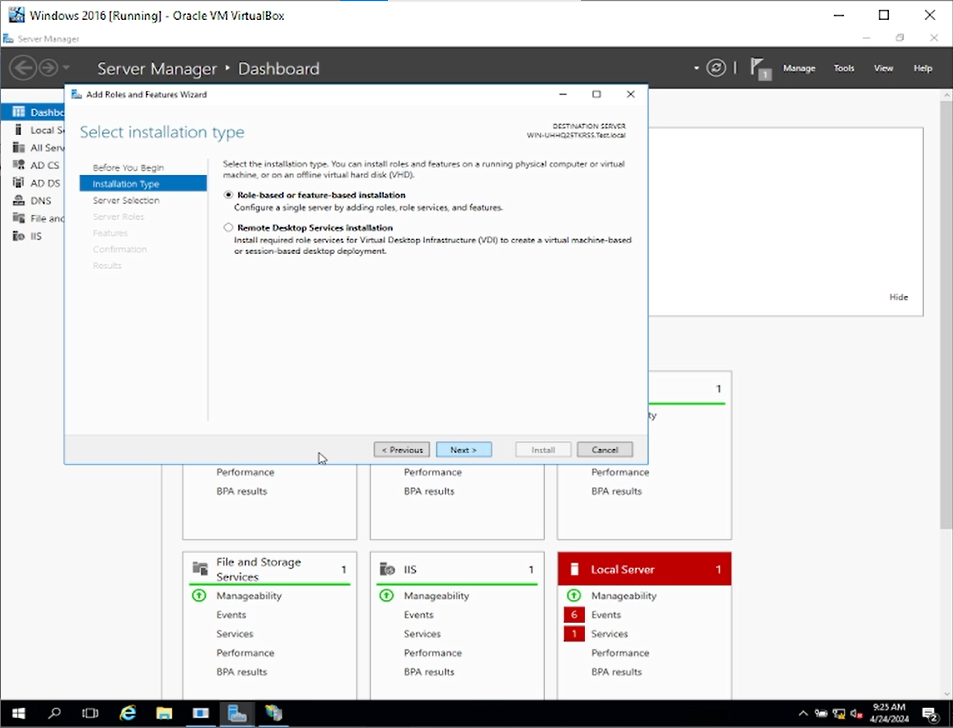
\includegraphics[width=0.8\linewidth]{figure//chapter9//lab9_2/installation-type.png}
    \caption{Chọn loại cài đặt}
    \label{fig:enter-label}
\end{figure}

\newpage

\noindent {\bf{Bước 6:}} Ở trang \textbf{Select destination server}, chọn \textbf{Select a server from the server pool}. Chọn server của bạn.

\begin{figure}[!htb]
    \centering
    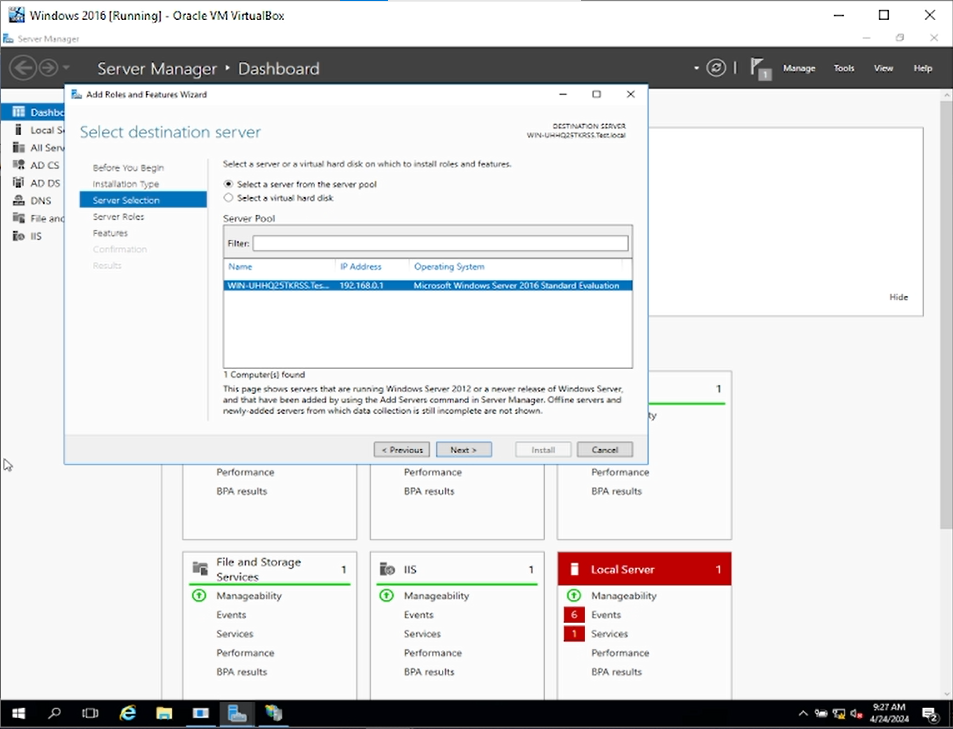
\includegraphics[width=0.8\linewidth]{figure//chapter9//lab9_2/destination-server.png}
    \caption{Chọn Destination server}
    \label{fig:enter-label}
\end{figure}

\noindent {\bf{Bước 7:}} Tới trang \textbf{Select server roles}, mở rộng \textbf{Web Server (IIS) và FTP Server}. Chọn \textbf{FTP Server} và \textbf{FTP Service}. Tiếp tục rồi chọn \textbf{Install}.

\begin{figure}[!htb]
    \centering
    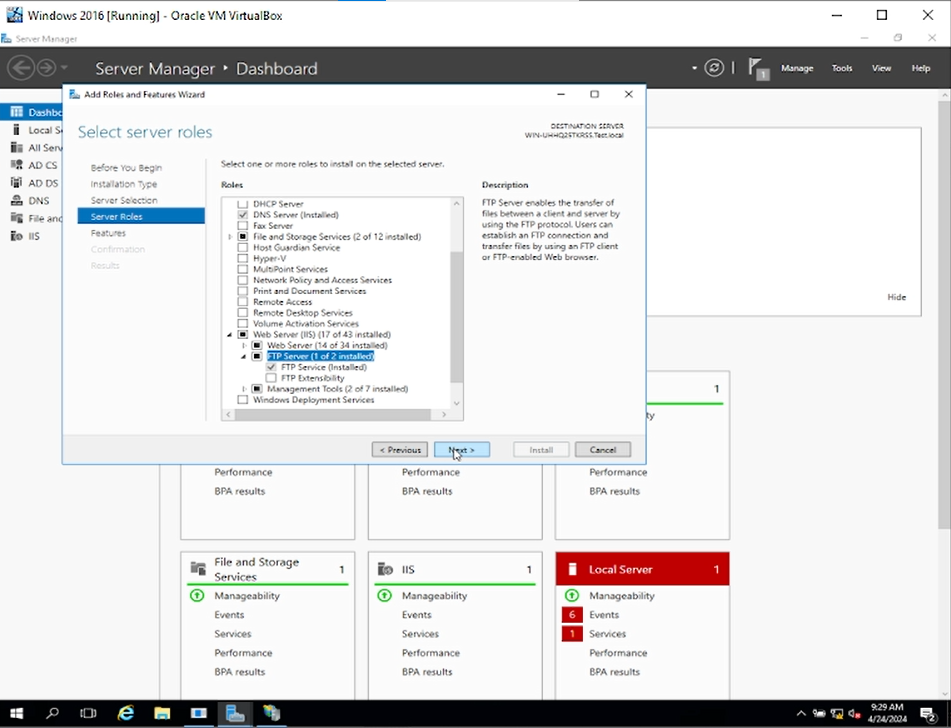
\includegraphics[width=0.8\linewidth]{figure//chapter9//lab9_2/select-role.png}
    \caption{Chọn server roles}
    \label{fig:enter-label}
\end{figure}

\noindent {\bf{Bước 8:}} Tạo folder tên là \textbf{FTP Data}, rồi tạo tệp \textbf{Credentials.txt} trong folder đó rồi lưu vào ổ C. Nội dung tệp là tên của bạn và ngày tháng hiện tại.

\begin{figure}[!htb]
    \centering
    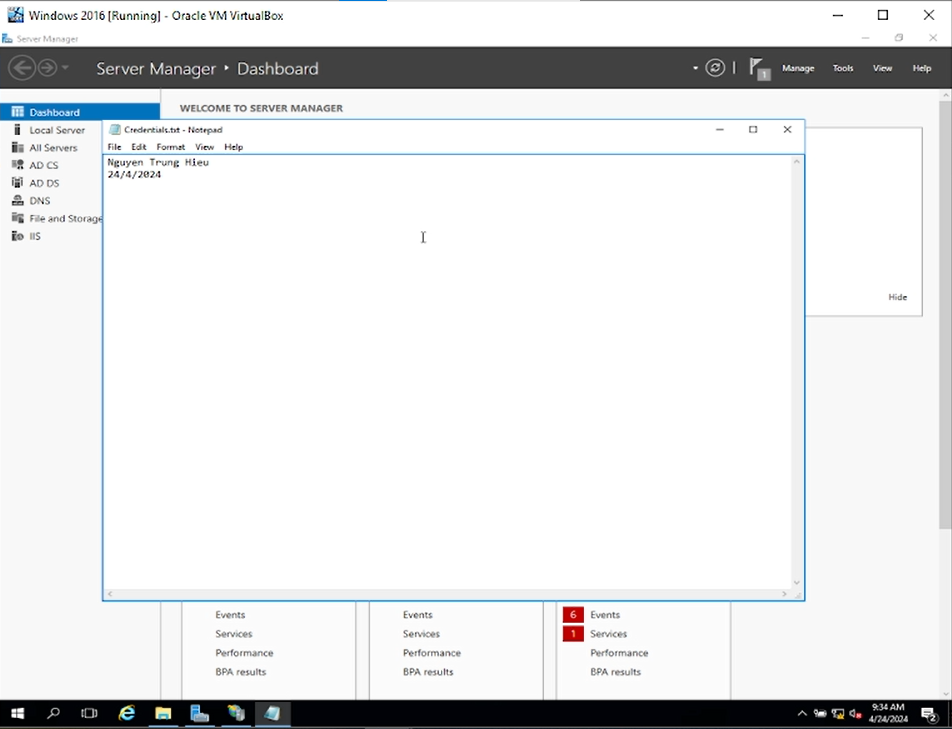
\includegraphics[width=0.75\linewidth]{figure//chapter9//lab9_2/create_file.png}
    \caption{Tạo file Credentials.txt}
    \label{fig:enter-label}
\end{figure}

\noindent {\bf{Bước 9:}} Ở IIS Manager, mở rộng \textbf{Windows Server}, chuột phải vào \textbf{Sites} và chọn \textbf{Add FTP site}. Đặt tên site là \textbf{FTP Data}, và nhập đường dẫn vật lý tới folder \textbf{FTP Data} vừa tạo.

\begin{figure}[!htb]
    \centering
    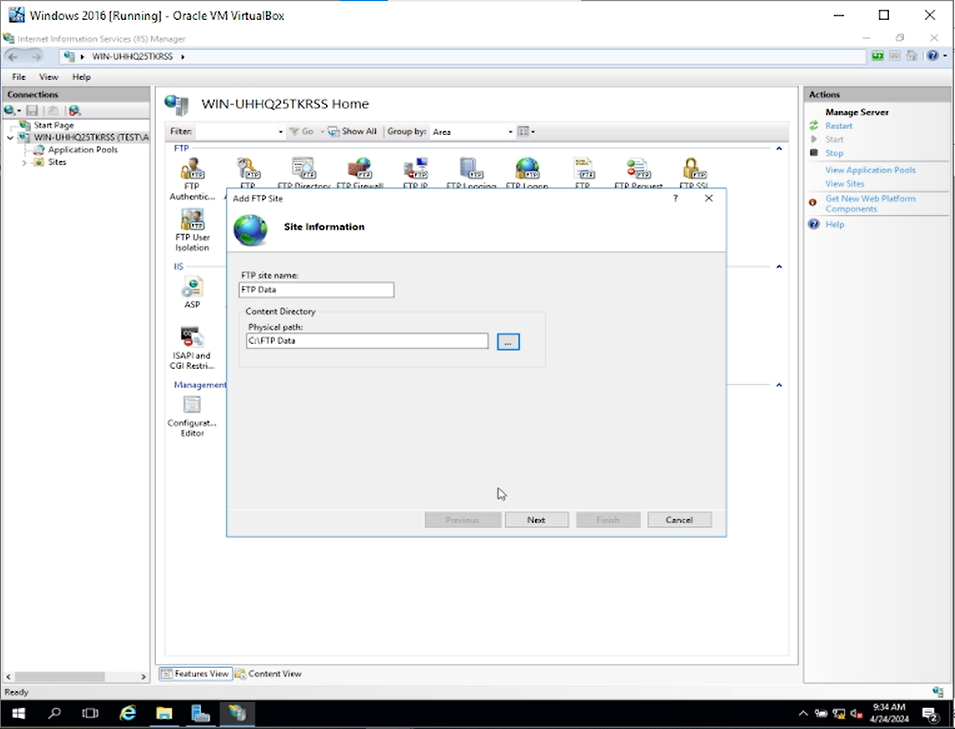
\includegraphics[width=0.8\linewidth]{figure//chapter9//lab9_2/create_ftp_site_1.png}
    \caption{Tạo FTP site}
    \label{fig:enter-label}
\end{figure}

\noindent {\bf{Bước 10:}} Ở trang \textbf{Bindings and SSL Settings}, ở phần IP address, chọn địa chỉ IP của bạn. Chọn \textbf{No SSL}.

\begin{figure}[!htb]
    \centering
    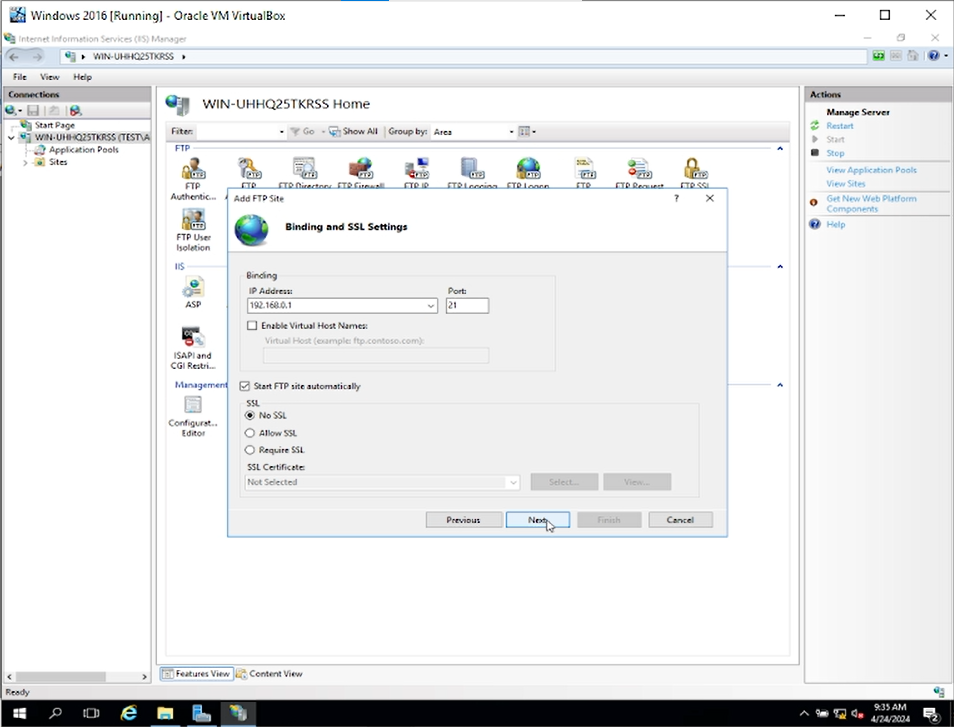
\includegraphics[width=0.8\linewidth]{figure//chapter9//lab9_2/ssl_settings.png}
    \caption{Cấu hình binding và SSL settings}
    \label{fig:enter-label}
\end{figure}

\noindent {\bf{Bước 11:}} Ở phần \textbf{Authentication}, chọn \textbf{Anonymous} và \textbf{Basic}. Còn ở \textbf{Authorization} thì chọn \textbf{All users}.

\begin{figure}[!htb]
    \centering
    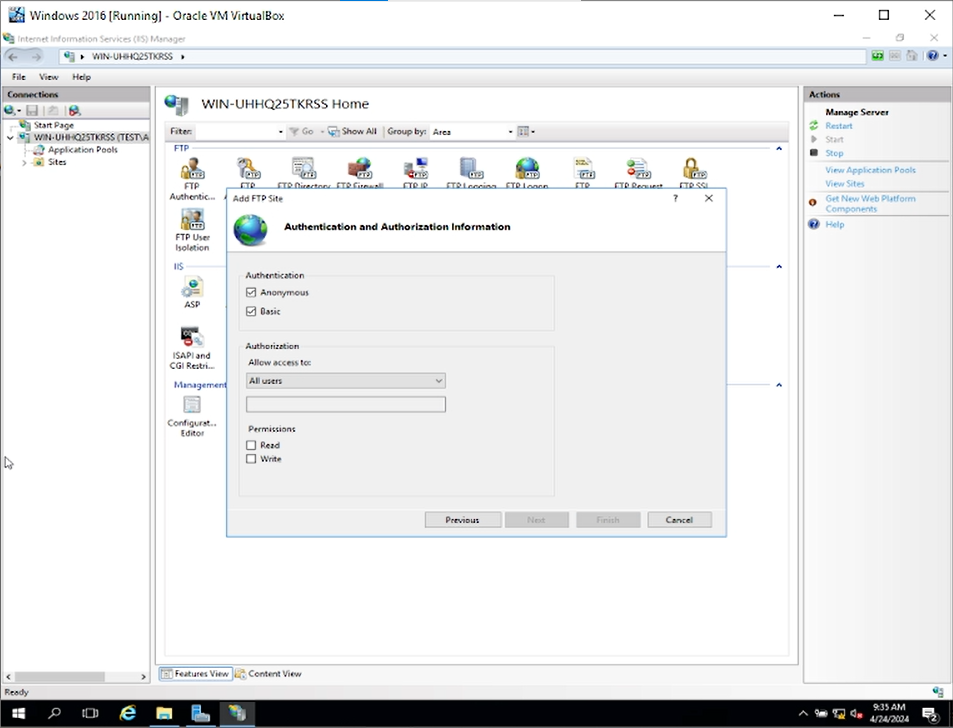
\includegraphics[width=0.8\linewidth]{figure//chapter9//lab9_2/auth.png}
    \caption{Cấu hình Authentication và Authorization}
    \label{fig:enter-label}
\end{figure}

\newpage

\noindent {\bf{Bước 12:}} Ở \textbf{Search box}, tìm \textbf{wf.msc} rồi tắt tường lửa với cả \textbf{Domain}, \textbf{Public} và \textbf{Private}.

\begin{figure}[!htb]
    \centering
    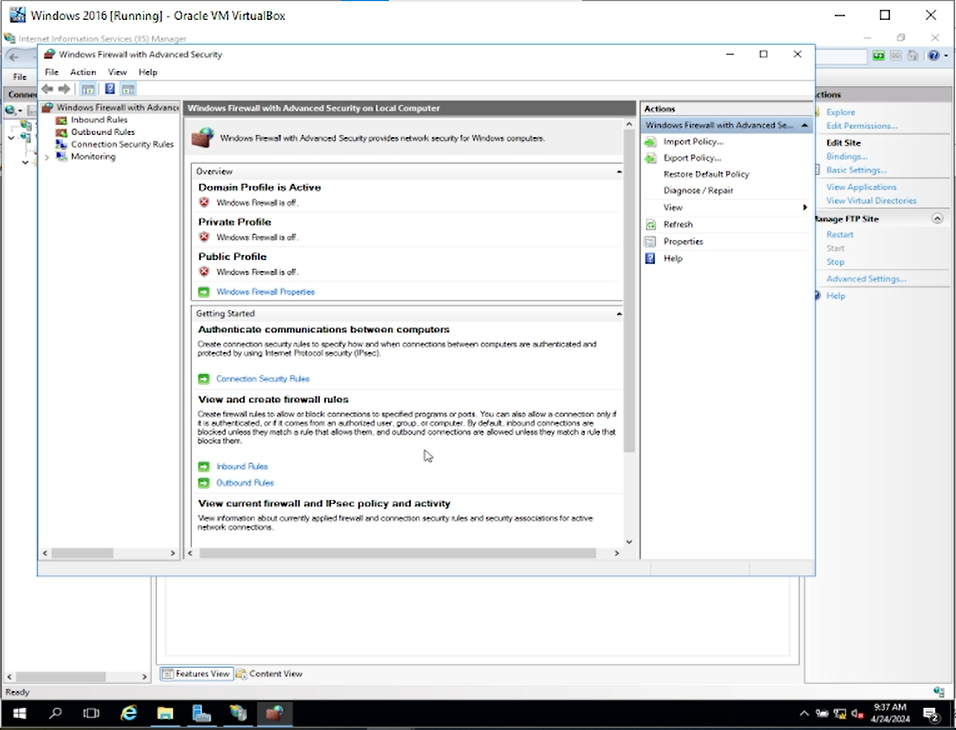
\includegraphics[width=0.85\linewidth]{figure//chapter9//lab9_2/turn_off_fw.png}
    \caption{Tắt tường lửa}
    \label{fig:enter-label}
\end{figure}

\noindent {\bf{Bước 13:}} Mở Windows 10 VM, truy cập \href{https://www.wireshark.org/download.html}{Link} để tải wireshark cho Windows.

\begin{figure}[!htb]
    \centering
    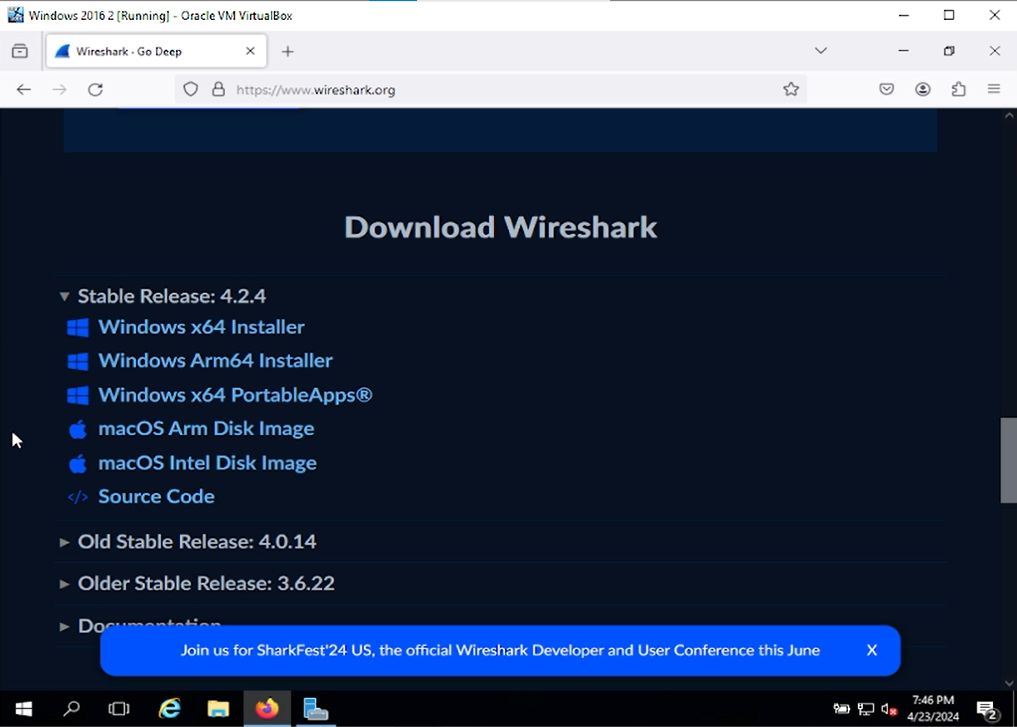
\includegraphics[width=0.9\linewidth]{figure//chapter9//lab9_2/download_wireshark.png}
    \caption{Tải Wireshark trong Windows}
    \label{fig:enter-label}
\end{figure}

\noindent {\bf{Bước 14:}} Cài đặt Wireshark, chấp nhận các cài đặt mặc định.

\begin{figure}[!htb]
    \centering
    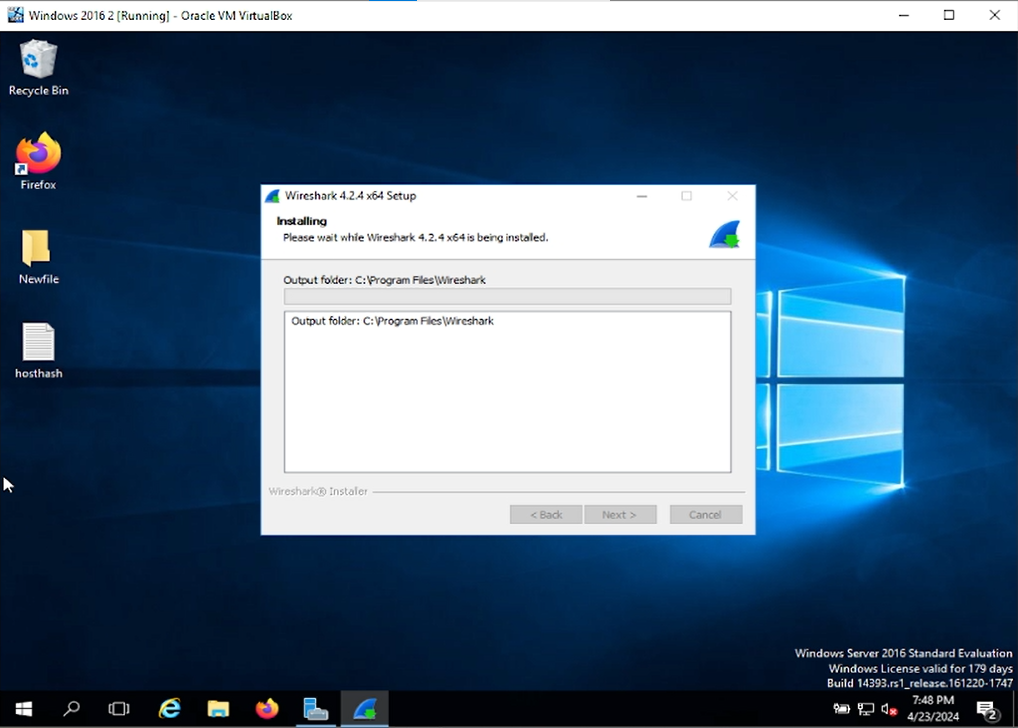
\includegraphics[width=0.9\linewidth]{figure//chapter9//lab9_2/install_wireshark.png}
    \caption{Cài đặt Wireshark}
    \label{fig:enter-label}
\end{figure}

\noindent {\bf{Bước 15:}} Cài đặt Npcap, đồng ý với các cài đặt mặc định.


\begin{figure}[!htb]
    \centering
    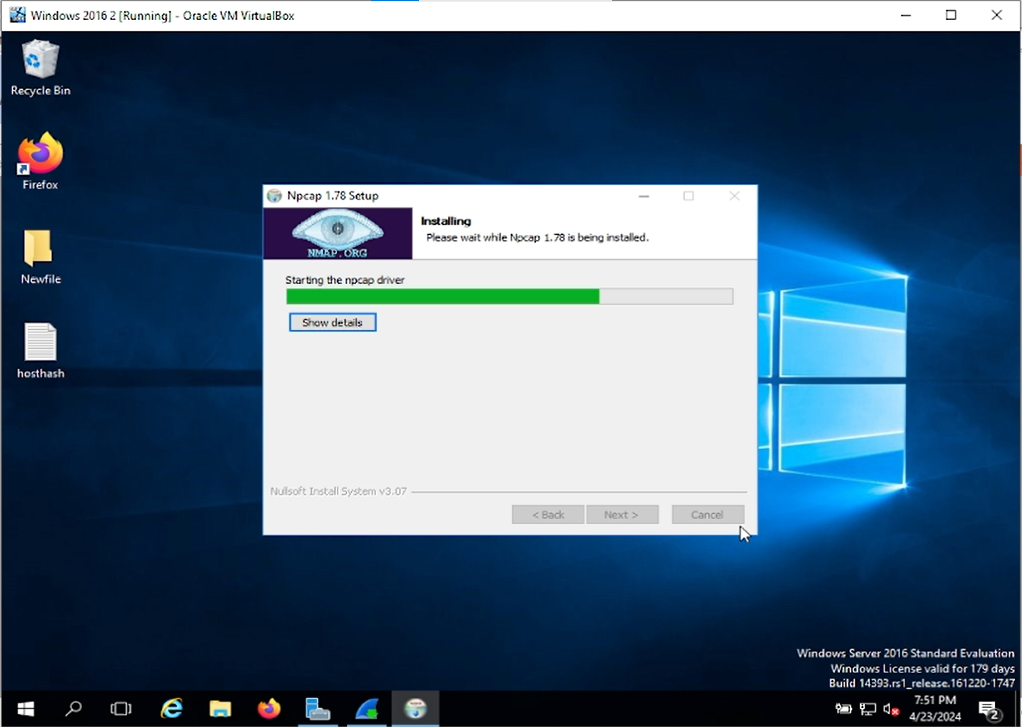
\includegraphics[width=0.9\linewidth]{figure//chapter9//lab9_2/install_npcap.png}
    \caption{Cài đặt Npcap}
    \label{fig:enter-label}
\end{figure}

\subsection{Review Questions}

\noindent Câu 1:

B: Users from the Internet have accessed your FTP server.

\noindent Câu 2: 

A: Microsoft Network Monitor captures.

D: Tcpdump.

\noindent Câu 3: 

B: WinPcap allows applications to capture and transmit network packets bypassing the protocol stack.

\noindent Câu 4: True.

\noindent Câu 5:

C: Microsoft IIS Log File Format.